\chapter{System implementation with Robot controller module}
\indent This chapter describes how all of components mentioned above are assembled. In design, I apply top-down approach in system development process. First, system is broken down into modules in which each system's function is handled separately. Next, functions of modules are presented in groups of communicating interfaces and groups of internal processing methods. Consequently, modules is divided into smaller and more dedicated units.

For each module, design pattern is engaged correspondingly to its operation behavior for the sake of ease in maintenance and convenience for extensibility.

Finally, when the system walking through all unit test cases, it is connected with the Delta robot to accomplish desired activities.

\section{System implementation}
\subsection{Whole system class diagram}
Figure \ref{fig:class_diagram} mentions all system ``workers'' known as classes \footnote{For convenient mentioning, interfaces are included}. These classes are organized in hierarchy and has relationship with each other. Some are compositions. Some are inheritances. Some have references to another classes. The detail of class relationships will be explained in upcoming sections.

    \begin{figure}[H]
		\centering
		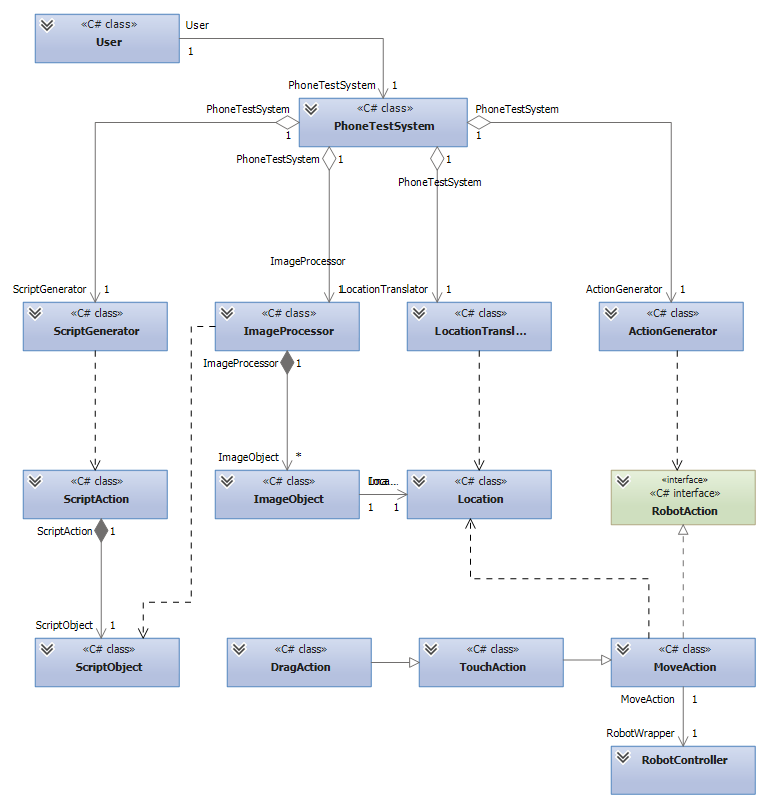
\includegraphics[scale=0.75]{Chapters/Fig/class_diagram.png}
		\caption{System class diagram}
		\label{fig:class_diagram}
	\end{figure}

\subsection{Main components of the system}
System consists of 3 main modules, which are Image Processing module, Script Managing module and Robot Action Handling module. Image Processing module involves in detecting and recognizing screen elements along with managing and organizing them for further access. Script Managing module does the job of operating test cases. Robot Handling module defines the movements of the robot and proposes inducing methods to other components so as to have the robot working.

	\begin{figure}[H]
		\centering
		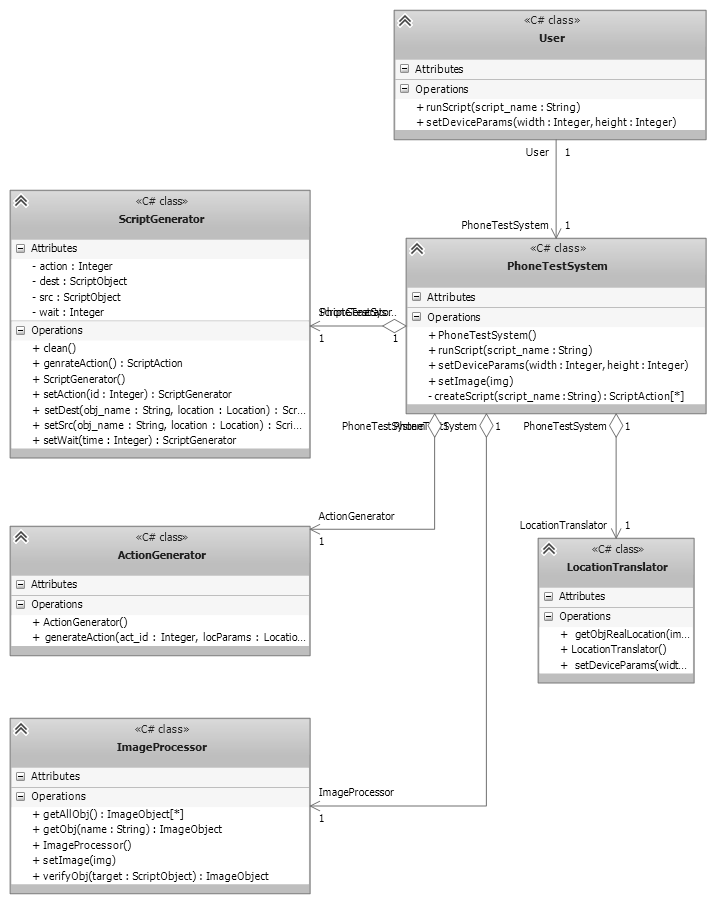
\includegraphics[scale=0.75]{Chapters/Fig/main_class.png}
		\caption{System main components}
		\label{fig:main_class}
	\end{figure}

There are also some assisting classes. PhoneTestSystem takes responsibility for wrapping up all modules and provide interface functions to user. LocationTranslator holds user input parameters with the purpose of converting actual phone screen location into pixel location in screen image and vice versa.

\subsection{Image Processor structure}
Using image processing technique presented in Chapter \ref{ch:screen_recognize}, screen elements are wrapped into objects which has name and location relatively to the screen reference system.

	\begin{figure}[H]
		\centering
		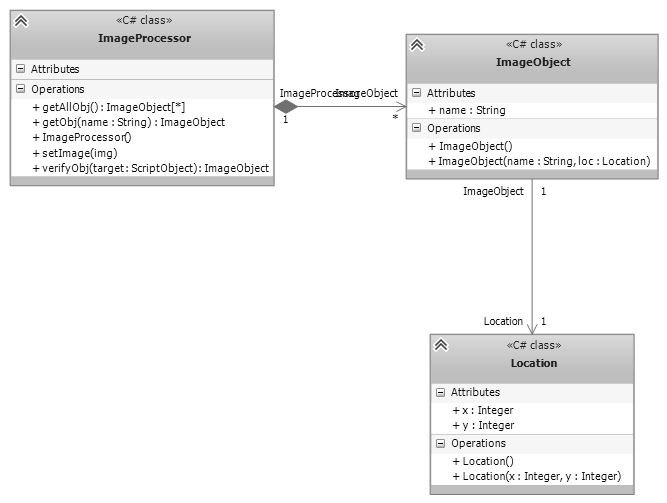
\includegraphics[scale=0.75]{Chapters/Fig/img_processor.png}
		\caption{Image Processor structure}
		\label{fig:img_processor}
	\end{figure}

An ImageProcessor receive image input from outer classes and parse its content into list of managed objects called ImageObjects. An ImageObject holds target's name which is text read from screen, and location in percent with screen coordinate. The location can be used for converting to real location later via LocationTranslator mentioned above. The name of object is used for searching and verifying element in script through \textit{getObj} and \textit{verifyObj} methods of ImageProcessor.

\subsection{Script Generator structure}
A script is formed of sequence of actions which are introduced in Section \ref{sec:script_comp}. Considering that each action can have different members but shares some required factors, ScriptGenerator is inspired by ``Builder Pattern'' \footnote{Read more at: \url{http://www.oodesign.com/builder-pattern.html}} to allow a dynamic way to generate script action on demand.

	\begin{figure}[H]
		\centering
		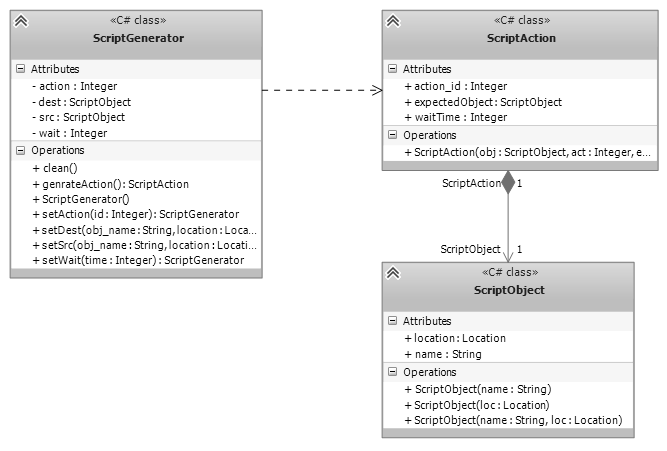
\includegraphics[scale=0.75]{Chapters/Fig/script_gen.png}
		\caption{Script Generator structure}
		\label{fig:script_gen}
	\end{figure}

Corresponding to each attribute of a script action, there is a \textit{set} method. Depending on situation, appropriate method is called. For an example, in Figure \ref{fig:click_test_diag}, a simple action like Clicking on READY button only needs a target and action type (click, in this case). Thus, two methods ``setSrc'' and ``setAction'' are called and finished with ``generateAction'' method to produce an instance of ScriptAction. Another case is Clicking on SUCCESS button. This action require a result to be verified which is READY button. Hence, destination object need to be set by ``setDest'' method before ``generateAction'' being called. By using this kind of pattern, attributes of desired object are built intentionally.

\subsection{Action Generator structure}
ActionGenerator is in charge of providing an interface for telling the robot what to do. The actions of the robot are represented in 3 basic classes. Figure \ref{fig:act_gen} describes the relation between these classes.

	\begin{figure}[H]
		\centering
		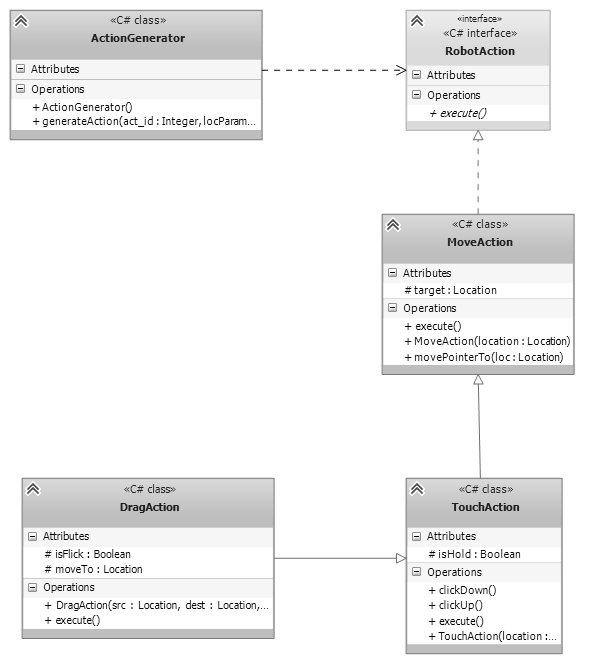
\includegraphics[scale=0.75]{Chapters/Fig/act_gen.png}
		\caption{Action Generator structure}
		\label{fig:act_gen}
	\end{figure}

Based on ``Command Pattern'' \footnote{Read more at: \url{http://www.oodesign.com/command-pattern.html}}, action request is encapsulated in an object that allows the parameterization with different requests. The client simply calls \textit{execute} method of a RobotAction instance and let it run itself. The execution detail is predefined at action's initialization through ActionGenerator.

The most basic movement is moving the robot's pointer. When this action is executed, the pointer will be move to chosen location. The following actions, such as Touch, Drag, Long Click and Flick, are derived from this action and then compose more complex movements.

\section{Robot interface command}

	\begin{itemize}
		\item[--] GotoXYZ
		\item[--] GotoTarget
		\item[--] ClickUp
		\item[--] ClickDown
	\end{itemize}
